\documentclass[letterpaper,12pt]{article}

\usepackage[utf8]{inputenc}
\usepackage{wasysym}
\usepackage{CJK}
\usepackage{graphicx}

%opening
\title{Open Source Software Engineering}
\author{Wilson High School}

%title page

\begin{document}

\begin{titlepage}
\begin{center}
 ~\\[1cm]
 \textsc{\LARGE Software Development}\\[1.5cm]
 \textsc{\Large TSA Regional Competition}\\[0.5cm]
 \rule{\linewidth}{0.5mm}
 {\huge \bfseries Shogi AI and Client \\[0.4cm]}
 \rule{\linewidth}{0.5mm}\\[0.5cm]
 \begin{CJK}{UTF8}{gbsn}
 {\huge 将棋}
 \end{CJK}
 \vfill
 {\large Lancaster, PA \\[0.4cm]}
 {\large 7 February 2015}
\end{center}
\end{titlepage}

\tableofcontents

\pagebreak

\section{Research}

Our research was focused on the rules and gameplay of shogi, the Japanese analogue of chess. The goal of the game, as with the familiar version of chess, is to place the opponent's king in checkmate. The game is played on a nine-by-nine board with eight kinds of pieces:

\begin{itemize}
 \item Pawns move forward one square at a time
 \item A king can move one square in any direction, although it is subject to being placed in check and suffers the associated restrictions the same way as a king from chess 
 \item Gold generals can move one square in any direction except diagonally backwards
 \end{itemize}

 \begin{center}
  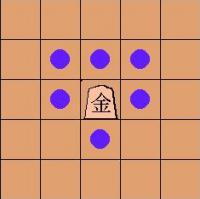
\includegraphics[width=5cm]{img/goldMove.jpg}
 \end{center}
 
 \begin{itemize}
  \item Silver generals can move straight or diagonally forward, as well as diagonally backwards
 \end{itemize}
 
 \begin{center}
  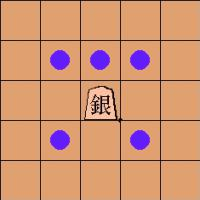
\includegraphics[width=5cm]{img/silverMove.jpg}
 \end{center}
  
 \begin{itemize}
  \item A knight moves forward two spaces and one space to the side, jumping over any intervening pieces, mimicking the motion of its chess counterpart except for its inability to move sideways or backwards
 \end{itemize}
 
 \begin{center}
  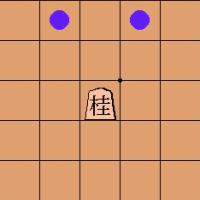
\includegraphics[width=5cm]{img/knightMove.jpg}
 \end{center}
 
 \begin{itemize}
  \item A lance moves any number of open spaces straight forward
  \item A rook moves any number of open spaces forward, backward, or to the sides
  \item A bishop moves any number of open spaces in any diagonal direction
 \end{itemize}
 
 In addition to the original pieces are promoted pieces. Promotion is a feature of shogi similar to pawn promotion in standard chess, but each piece has a specified promotion. Two pieces (the king and the gold general) are not promoted at all if the conditions are met. Promotion may occur when a piece moves into any space among the far three rows of the board, although a piece does not have to be promoted if the player doesn’t want to. Promoted pieces move as follows:
  \begin{itemize}
  \item A promoted pawn, silver general, knight, or lance moves as if it were a gold general.
  \item A promoted rook or bishop gains the ability to move one square in the directions it couldn’t prior to the promotion (so a promoted rook would be able to move one space diagonally, and a bishop could move one space vertically or horizontally)
  \end{itemize}

Pieces are captured when one piece moves into a square occupied by an opposing piece, just like in chess. A piece’s promotion is lost upon being captured.

In addition to promotion, shogi adds another unique mechanic: “drops.” A drop is when the player places a piece previously captured from her opponent somewhere on the board. A drop takes a full turn, and the only restrictions on it are that a piece cannot be dropped somewhere it would be unable to move the next turn (so, a pawn cannot be dropped into the back row), and a player may not place a pawn in such a way that he will have two in the same column. A piece cannot be promoted by dropping it into the back three rows, and a piece loses its promotion when captured, so a piece will never be promoted on the turn it is dropped. After the drop the piece acts as it normally would, following all the rules as if it had moved to its current location normally.

The shogi board is laid out as follows, on a 9x9 board.

\begin{center}
 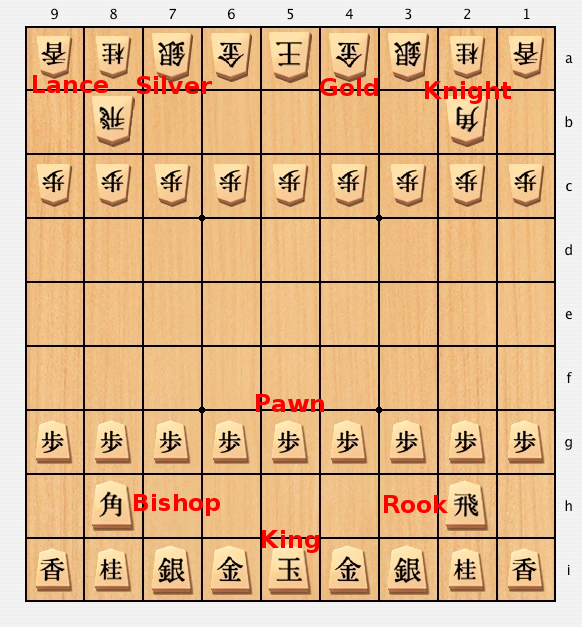
\includegraphics[width=10cm]{img/shogiBoard.png}
\end{center}

\section{Overview}
The main goal of the Shogi AI project is to provide an educational environment for newcomers to learn how to play the game. In summary, we hope to accomplish this by providing a few elements:
\begin{itemize}
 \item Graphical User Interface for move input
 \item Varying levels of Shogi AI to play against
 \item Game commentary provided by an AI
\end{itemize}
In future versions, we hope to include:
\begin{itemize}
 \item Server integration so the user can play against opponents across the globe.
 \item Advanced AI that can challenge and beat the best players
 \item Shogi variants to mix up play
\end{itemize}

\newpage

\section{Documentation}

\subsection{Project Requirements}

\subsection{Software Design}

\subsection{Testing}

\subsection{User Manual}

\section{Evaluation}

\section{Bibliography}

\end{document}
